 \documentclass[rgb]{beamer}
\usepackage{silence,lmodern}
\usepackage[backend=biber, style=nature]{biblatex}
\usepackage{csquotes}
\usepackage{listings}
\usepackage{svg}
\usepackage{multirow}
\usepackage{booktabs}
\usepackage{multicol}
\usepackage{forest}
\usepackage[format=plain, justification=justified, labelfont=bf, textfont=it, font=small, labelsep=space]{caption}
\usepackage{appendixnumberbeamer}

\WarningFilter{biblatex}{Patching footnotes failed}
\WarningFilter{etex}{Extended allocation already in use}

\renewcommand*{\bibfont}{\tiny}
\bibliography{resources.bib}

\usetheme{Konstanz}
\setcounter{secnumdepth}{3}
\format{169}


\title{Locality Optimization for traversal-based Queries on Graph Databases}
\titleCorporateDesign{Locality Optimization}{for traversal-based}{Queries on}{Graph Databases}
\author{Fabian Klopfer} 
\date{30.04.2021}
\institute{Databases and Information Systems Group \\ Department of Computer and Information Science \\ University of Konstanz}

\AtBeginDocument{
\usebeamerfont{normalfont}
\begin{frame}
	\titlepage
\end{frame}
}

\begin{document}
  \begin{frame}<beamer>
    \frametitle{Outline}
    \tableofcontents[subsectionstyle=hide]
  \end{frame}
  
\section{Introduction}
        \begin{frame}[allowframebreaks]{Motivation}
        Current state of performance-optimized \\ [0.5em]
        \begin{itemize}
            \item relational databases:
            \begin{itemize}
                \item Storage order determined by join attribute.  $\rightarrow$ enables localized access.
                \item Explicit clustered indices (often B+-Trees). $\rightarrow$ represents order, speeds up range queries
            \end{itemize}
            $\Rightarrow$ Accesses are made as sequential as possible. \\
            [1em]
            
            \item graph databases:
            \begin{itemize}
                \item Storage order determined by insertion order.
                \item Implicit, possibly unclustered index for relationships (doubly-linked list).
                \item Lucene-based indexes on properties, labels, $\dots$, unclustered.
            \end{itemize}
            $\Rightarrow$ Access is mostly random.
        \end{itemize}
    \end{frame}
    
    \begin{frame}[allowframebreaks,fragile]{Example}
        Show me all boats owned by sailors with an ID less than 50:
        
        \begin{figure}[htp]
        \begin{center}
        \begin{forest}
            [ $\quad \bowtie^m$
            [ $\quad \bowtie^m$
                [ index $\sigma_{\text{ID} < 50}$ S ]
                [ scan O ]
            ]
            [ scan B ]
        ]
        \end{forest} 
        \end{center}        
        \end{figure}
        Reads are mostly sequential. \\   
        $\Rightarrow$ Prefetch \& cache hit.
        
        \framebreak
        
        Nodes are Sailors and Boats, relationships ``owns''
        
        \begin{figure}[htp]
        \begin{center}
          \begin{forest}
            [ $\sigma_{y.\text{label = Boat}}$
            [ $\uparrow_x^y$
                [ $\sigma_{x.ID < 50}$ ($\bigcirc$ x) ]
            ]
        ]
        \end{forest} 
        \end{center}        
        \end{figure}
        Scaning and filtering is sequential. \texttt{Expand} is not. \\ 
        $\Rightarrow$ \texttt{Expand} causes prefetch \& cache misses.
                
            \framebreak
            
           % \includegraphics[keepaspectratio, height=0.8\textheight, width=\textwidth]{×}
            % TODO
            
            \begin{itemize}
            \item Especially \texttt{Expand} jumps a lot. Potentially back and forth. \\ [2em]
            \item Traversals rely primarily on expand. 
            \end{itemize}
    \end{frame}
        
        \section{Background}
            \subsection{Graphs}
                \begin{frame}{Graphs}
                    \begin{figure}
                     \begin{center}
                      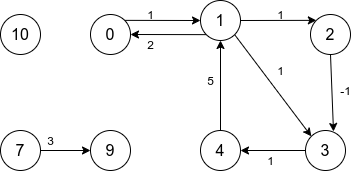
\includegraphics[keepaspectratio, height=0.8\textheight, width=0.6\textwidth]{img/data_struct_gr.png}
                     \end{center}
                    \end{figure}
                \end{frame}
            
                \begin{frame}{Traversals}
                    \begin{figure}
                     \begin{center}
                      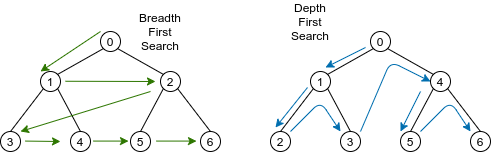
\includegraphics[keepaspectratio, height=0.8\textheight, width=0.8\textwidth]{img/bfs-dfs.png}
                     \end{center}
                    \end{figure}
                \end{frame}
                    
                
            \subsection{The Property Graph Model}
                \begin{frame}{Property Graph Model}
                    \begin{figure}
                     \begin{center}
                      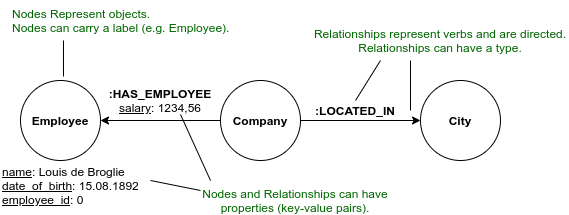
\includegraphics[keepaspectratio, height=0.8\textheight, width=.8\textwidth]{img/property_graph_elements.png}
                     \end{center}
                    \end{figure}
                \end{frame}
        
                \begin{frame}[allowframebreaks]{Data Structures}
                    Two essential record structures: \\ [2em]
                    \begin{enumerate}
                    \item Node records \\ [2em]
                    \item Relationship records
                    \end{enumerate}
                    
                    \framebreak
                    \begin{figure}
                     \begin{center}
                      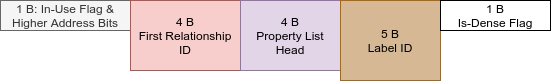
\includegraphics[keepaspectratio, height=\textheight, width=\textwidth]{img/node_record.png}
                     \end{center}
                    \end{figure}
                    
                    \framebreak
                    \begin{figure}
                     \begin{center}
                      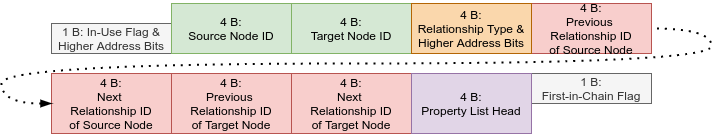
\includegraphics[keepaspectratio, height=\textheight, width=\textwidth]{img/relationship_record.png}
                     \end{center}
                    \end{figure}
                    
                    \framebreak
                    \begin{figure}
                     \begin{center}
                      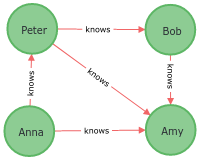
\includegraphics[keepaspectratio, height=0.6\textheight, width=.6\textwidth]{img/graph.png}
                     \end{center}
                    \end{figure}
                    \end{frame}
                    
                    \begin{frame}
                    \vspace{-3.5em}
                    \begin{figure}
                     \begin{center}
                      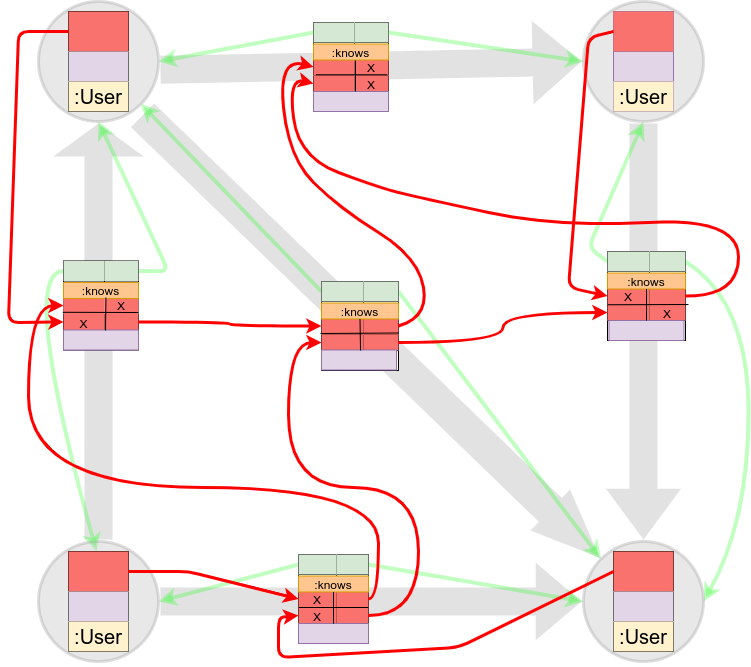
\includegraphics[keepaspectratio, height=1.2\textheight, width=\textwidth]{img/example_structs.png}
                     \end{center}
                    \end{figure}
                \end{frame}
        

    \section{Problem Definition}
        \begin{frame}[allowframebreaks]{Problem Definition}
            Given a graph $G$, logical block size $b$, page size $p$. \\ [2em]
            Desired is \\ [1em]
            \begin{enumerate}
            \item A partition of $G$ into blocks of vertex records $V_i$ and $E_i$ relationship records, \\ [1em]
            \item permutations $\pi_v, \pi_e$ of the blocks of vertex and edge records $V_i, E_i$,\\ [1em]
            \item a reordering of the incidence list pointers \\ [1.5em]
            \end{enumerate}
            such that spatial locality is as high as possible for traversal-based queries.
            
            \framebreak
            
             Temporal locality based on blocks.
                \[ P (X_{t + \Delta} = B | X_t = B) \]
            Spatial locality in the same sense:
                \[ P(X_{t + \Delta} = B \pm \varepsilon | X_t = B) \]
          
            \framebreak
            \begin{figure}[htp]
                \begin{center}
                    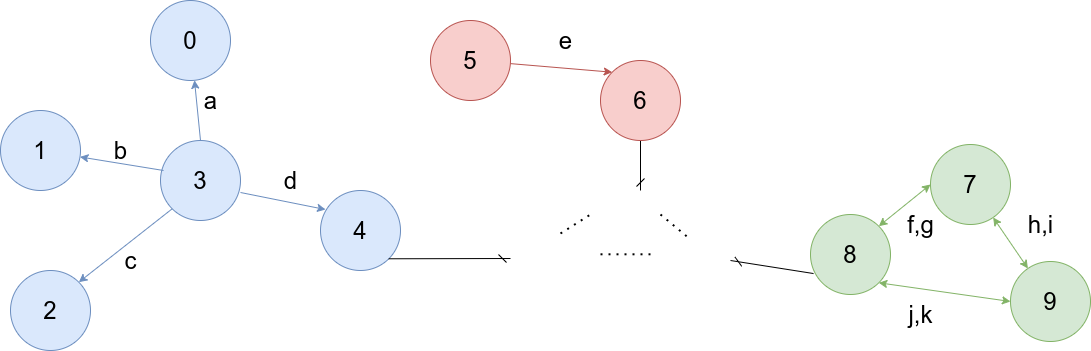
\includegraphics[keepaspectratio,height=0.4\textheight,width=\textwidth]{img/example_graph.png}
                \end{center}
            \end{figure}
            
             \begin{table}[htp]
                \centering
                \begin{tabular}[c]{|l|c|c|c|c|c|c|} \hline
                &&&&&&\\[-1em]
                node.db & \colorbox{blue!30}{0}, \colorbox{red!30}{5}, \colorbox{green!30}{7} & \colorbox{blue!30}{1}, \colorbox{blue!30}{4}, \colorbox{green!30}{9} & \colorbox{blue!30}{2}, \colorbox{red!30}{6}, \colorbox{green!30}{8} & \colorbox{blue!30}{3} &  & \\ \hline
                &&&&&&\\[-1em]
                edge.db & \colorbox{blue!30}{a}, \colorbox{green!30}{f} & \colorbox{blue!30}{b}, \colorbox{green!30}{g} & \colorbox{blue!30}{c}, \colorbox{green!30}{h} & \colorbox{blue!30}{d}, \colorbox{green!30}{i} & \colorbox{red!30}{e}, \colorbox{green!30}{j} & \colorbox{green!30}{k} \\  \hline
                \end{tabular}
                \vspace{0.5cm}
                
                \begin{tabular}{|l | c | c | c | c | c | c|} \hline
                &&&&&&\\[-1em]
                node.db & \colorbox{green!30}{7},\colorbox{green!30}{8}, \colorbox{green!30}{9} & \colorbox{blue!30}{0}, \colorbox{blue!30}{1}, \colorbox{blue!30}{3} & \colorbox{blue!30}{2}, \colorbox{blue!30}{4}, \colorbox{red!30}{5} & \colorbox{red!30}{6} &  & \\ \hline
                &&&&&&\\[-1em]
                 edge.db &  \colorbox{green!30}{f}, \colorbox{green!30}{h} & \colorbox{green!30}{g}, \colorbox{green!30}{k} & \colorbox{green!30}{i}, \colorbox{green!30}{j} & \colorbox{blue!30}{a}, \colorbox{blue!30}{b} & \colorbox{blue!30}{c}, \colorbox{blue!30}{d} & \colorbox{red!30}{e} \\ \hline
                \end{tabular}
            \end{table}
            
            \framebreak
            TODO insert incidence list chaos and ordered here
        \end{frame}
        
    \section{Locality-optimizing Record Layout}
        \begin{frame}[allowframebreaks, fragile]{G-Store}
            \begin{figure}[H]
                \begin{center}
                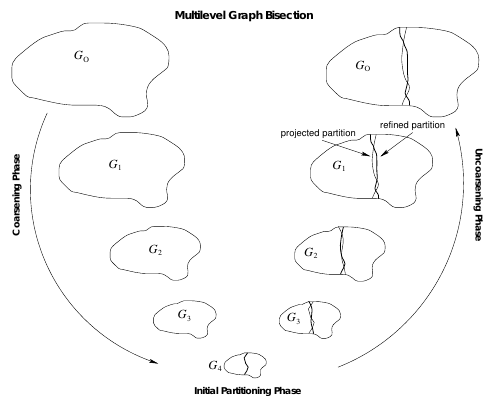
\includegraphics[keepaspectratio, height=0.8\textheight, width=\textwidth]{img/multilevel.png}\\
                \end{center}
            \end{figure}
            
            \framebreak
            \vfill\vspace{0pt}
            \begin{enumerate}
             \item Coarsening: Heavy-Edge Matching
             \item Turn-around
             \item Uncoarsening
                \begin{enumerate}
                 \item Project
                 \item Reorder
                 \item Refine
                \end{enumerate}
            \end{enumerate}
            
            \framebreak
            \begin{figure}[H]
                \begin{center}
                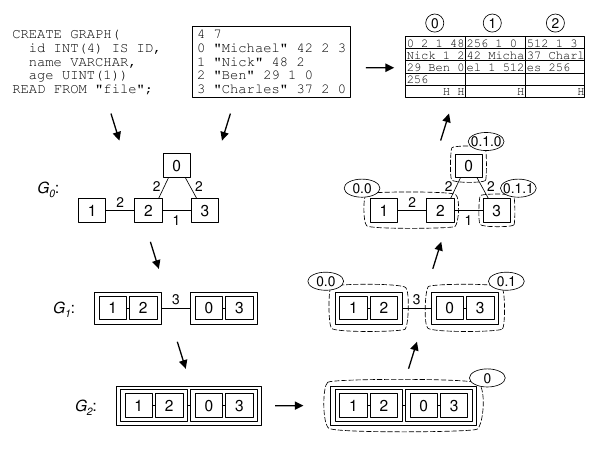
\includegraphics[keepaspectratio, height=0.9\textheight, width=\textwidth]{img/g-store.png}\\
                \end{center}
            \end{figure}
            \vfill\vspace{0pt}
        \end{frame}
        
        \begin{frame}[allowframebreaks]{ICBL}
        \vspace{-3.3em}
            \begin{figure}
                \begin{center}
                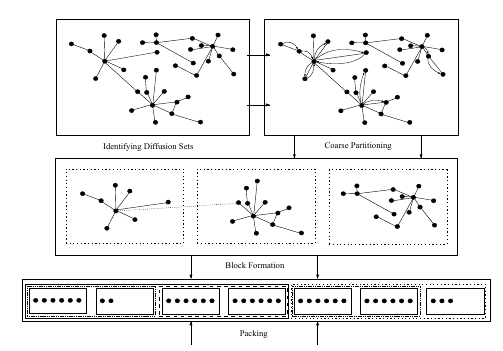
\includegraphics[keepaspectratio, height=\textheight, width=\textwidth]{img/icbl.png}
                \end{center}
            \end{figure}
            
            \framebreak
            \begin{enumerate}
             \item[I ] Feature extraction: Do $t$ random walks of length $l$. 
             \item[C] Coarse clustering: Adapted K-Means.
             \item[B] Block Formation: Agglomerative hierarchical clustering.
             \item[L] Layout Blocks: Sort blocks and subgraphs
            \end{enumerate}

            
        \end{frame}
        
        \begin{frame}[allowframebreaks]{Louvain Method}
            \begin{figure}
                \begin{center}
                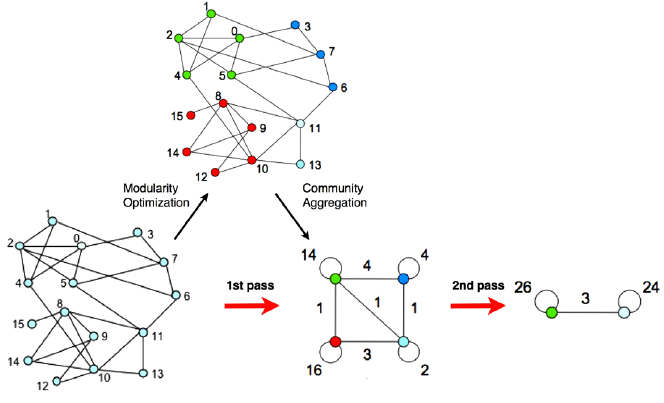
\includegraphics[keepaspectratio, height=0.8\textheight, width=.8\textwidth]{img/louvain.png}
                \end{center}
            \end{figure}
            
            \framebreak
            
            \begin{enumerate}
             \item Initialize all nodes in singleton community.
             \item Merge community into a neighboring community where modularity gain is maximal, until modularity gain is below threshold.
             \item Construct new graph from aggregated communities and go to 1.
            \end{enumerate}
            \vspace{2em}
            \[ Q = \frac{1}{2m} \sum_{u,v \in V} \left( w_{(u, v)} - \frac{w_u w_v}{2m} \right) \cdot \delta (c_u, c_v) \]
            
        \end{frame}
    
        \begin{frame}{Incidence List Rearrangement}
            \begin{enumerate}
             \item Traverse incidence list and store IDs.
             \item Sort IDs.
             \item Assign first relationship pointer to lowest ID.
             \item Assign next pointer of new first relationship to second ID.
             \item Assign next pointer of relationship $i$ to $i+1$. ID and prev pointer to $i-1$. ID.
             \item Assign next pointer of last relation to first and prev pointer of first to last.
            \end{enumerate}

        \end{frame}
        
    \section{Evaluation}
        \begin{frame}{Setup}
        \begin{itemize}
         \item Queries: BFS, DFS, Dijkstra, A$^*$, ALT. \\ [1em]
         \item Datasets: $[131, 1'134'890]$ nodes, $[764, 2'987'624]$ edges, average degree $[2.6, 25.5]$ \\ [1em]
         \item Domains include biological neural net, E-Mails, Co-authors, Frequent item sets, Comments.
        \end{itemize}
        \end{frame}
        
        \begin{frame}[allowframebreaks]{Results}
            \begin{figure}
                \begin{center}
                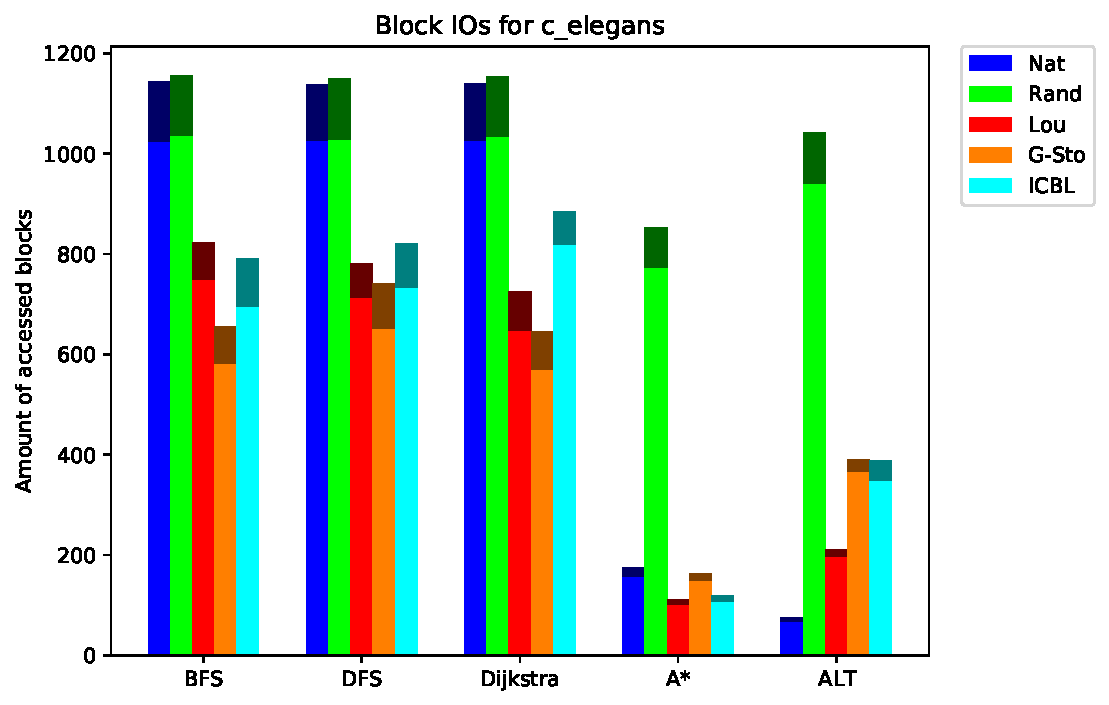
\includegraphics[keepaspectratio, height=0.8\textheight, width=\textwidth]{img/c_elegans_Block_unsorted_io_comparison.pdf}
                \end{center}
            \end{figure}
            
            \framebreak
            \begin{figure}
                \begin{center}
                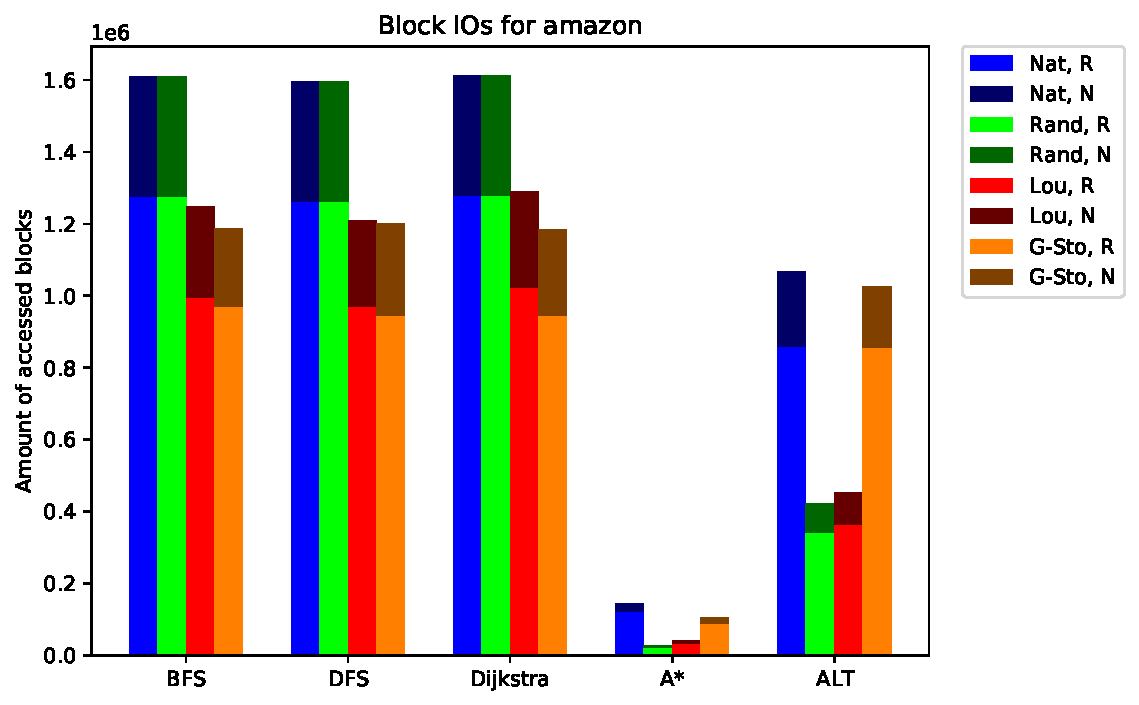
\includegraphics[keepaspectratio, height=0.8\textheight, width=0.48\textwidth]{img/amazon_Block_unsorted_io_comparison.pdf}
                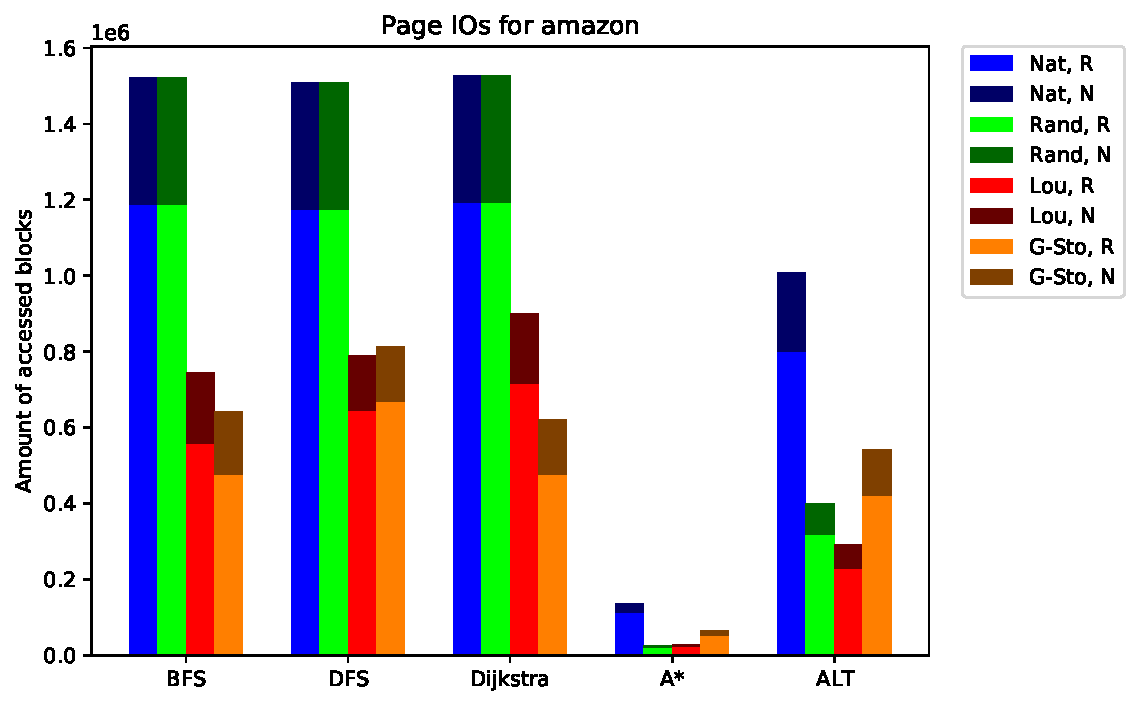
\includegraphics[keepaspectratio, height=0.8\textheight, width=0.48\textwidth]{img/amazon_Page_unsorted_io_comparison.pdf}
                \end{center}
            \end{figure}
            
            \framebreak
            \begin{figure}
                \begin{center}
                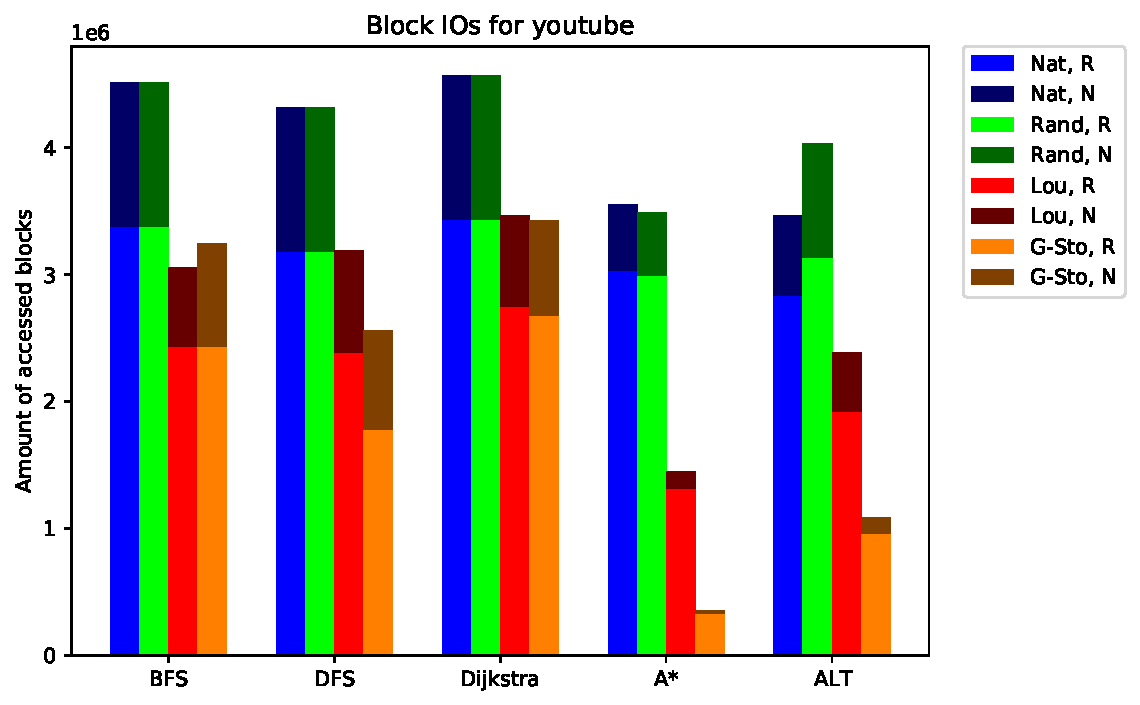
\includegraphics[keepaspectratio, height=0.8\textheight, width=\textwidth]{img/youtube_Block_unsorted_io_comparison.pdf}
                \end{center}
            \end{figure}
            
            \framebreak
            \begin{figure}
                \begin{center}
                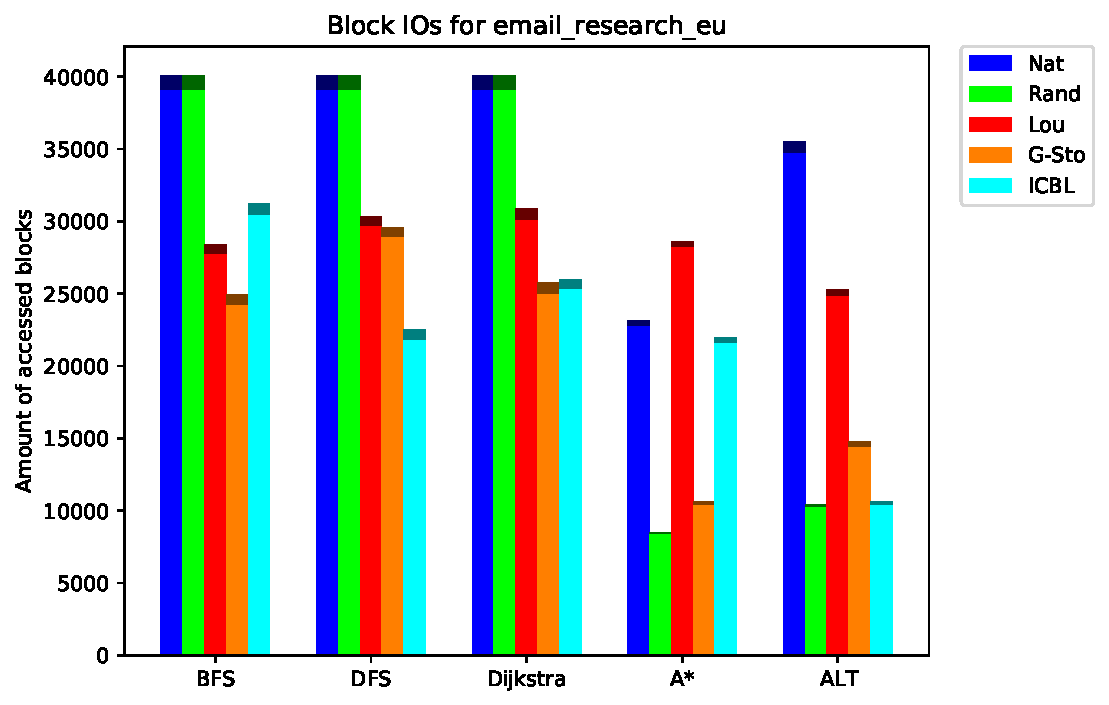
\includegraphics[keepaspectratio, height=0.8\textheight, width=\textwidth]{img/email_research_eu_Block_unsorted_io_comparison.pdf}
                \end{center}
            \end{figure}
            
            \framebreak
            \begin{figure}
                \begin{center}
                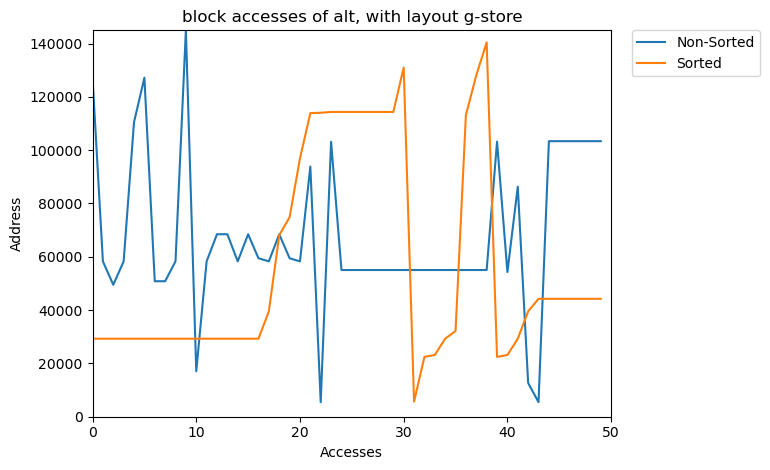
\includegraphics[keepaspectratio, height=0.8\textheight, width=\textwidth]{img/dblp_g-store_alt_block_sil_access_seq.png}
                \end{center}
            \end{figure}
            
            \framebreak
            \begin{figure}
                \begin{center}
                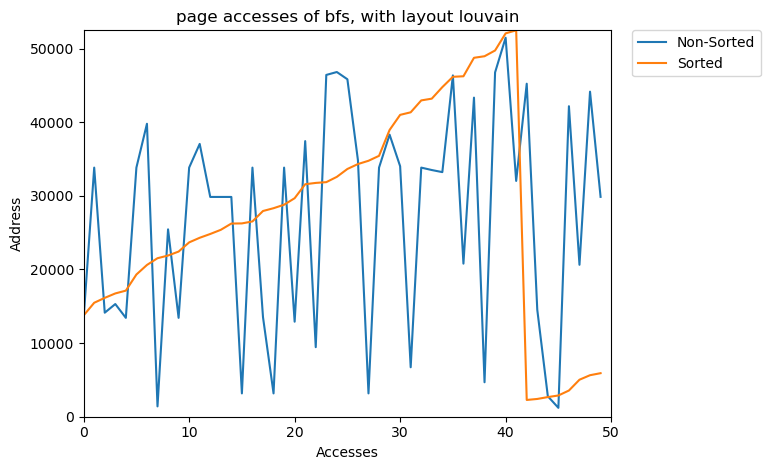
\includegraphics[keepaspectratio, height=0.8\textheight, width=\textwidth]{img/youtube_louvain_bfs_page_sil_access_seq.png}
                \end{center}
            \end{figure}
            
            \framebreak
            \begin{figure}
                \begin{center}
                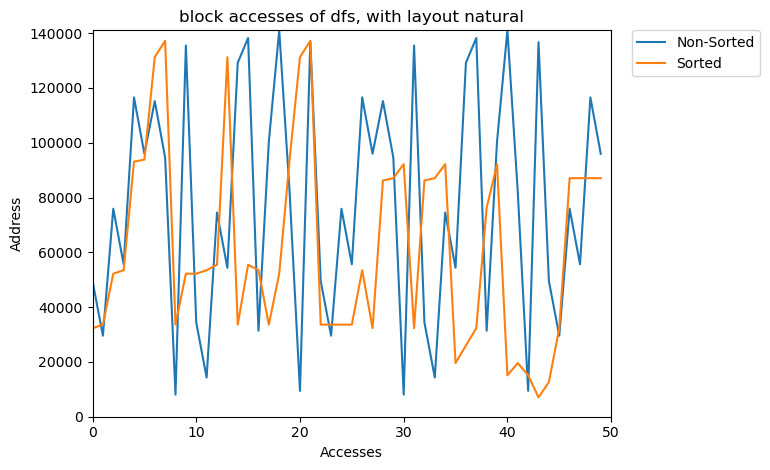
\includegraphics[keepaspectratio, height=0.8\textheight, width=\textwidth]{img/dblp_natural_dfs_block_sil_access_seq.png}
                \end{center}
            \end{figure}
        \end{frame}
    
    \section{Conclusion}
        \begin{frame}{Summary}
            \begin{itemize}
                \item Static rearrangement methods decrease number of block accesses. \\
                $\Rightarrow$ increase locality \\ [1em]
                \item Sorting the incidence lists leads to more sequential access sequences. \\ [1em]
                \item Ordering the blocks is crucial for spatial locality.
                \end{itemize}
        \end{frame}
    
        \begin{frame}{Future Work}
        \begin{itemize}
            \item Leiden instead of Louvain \\ [1em]
            \item RCM-based rearrangement \\ [1em]
            \item  Dynamic Rearrangement --- Query-based \\ [1em]
            \item Disk-based implementation
        \end{itemize}
        \end{frame}
        
    \printbibliography
\end{document}
